\documentclass[a4paper, 12pt]{report}
\usepackage[hidelinks]{hyperref}
\usepackage[a4paper, margin=2cm]{geometry}
\usepackage[english, russian]{babel}
\usepackage{graphicx}
\usepackage{wrapfig}
\usepackage{xcolor}
\usepackage{amsmath}
\usepackage{amssymb}


\setlength{\parindent}{0em}
\setlength{\parskip}{0pt}

\begin{document}

\begin{titlepage}
    \begin{center}
    \textsc{Министерство науки и высшего образования Российской Федерации \\
    ФЕДЕРАЛЬНОЕ ГОСУДАРСТВЕННОЕ АВТОНОМНОЕ ОБРАЗОВАТЕЛЬНОЕ УЧРЕЖДЕНИЕ ВЫСШЕГО ОБРАЗОВАНИЯ НАЦИОНАЛЬНЫЙ ИССЛЕДОВАТЕЛЬСКИЙ УНИВЕРСИТЕТ ИТМО \\[5mm]
    }

    \vfill
    \vfill

    \textbf{
    \Large{Лабораторная работа №5
    по дисциплине} \\
    \Large{“Статистика и анализ данных” }
    \\[6mm]
    Семестр 2
    \\[20mm]
    }
    \end{center}

    \hfill
    \begin{minipage}{.5\textwidth}
    \begin{flushright}
    Выполнили студенты:\\[2mm] 
    Косарев Илья, \\
    гр. J3110, ИСУ 466304\\[2mm]

    Капустина Юлия, \\
    гр. J3110, ИСУ 466110\\[2mm]

    Кащеев Максим,\\
    гр. J3111, ИСУ 466147\\[3mm]
    Отчет сдан: \\
    19.05.2025


    \end{flushright}
    \end{minipage}%
    \vfill
    \begin{center}
    Санкт-Петербург,\\
    2025 г.
    \end{center}
\end{titlepage}

\tableofcontents
\newpage

\chapter*{Введение}
\addcontentsline{toc}{chapter}{Введение}
\setcounter{chapter}{1}
\setcounter{section}{0}

\section{Цель и задачи}
\textbf{Цель}: познакомиться с понятием временного ряда и применить различные методы анализа к данному. \par
\textbf{Задачи}:
\begin{enumerate}
    \item Импортировать временной ряд для анализа (в данной работе в качестве такого ряда был взят
    временной ряд цен закрытия акций \textit{MSFT});
    \item построить разностные ряды различного порядка;
    \item построить автокорреляционную функцию ряда и провести анализ трендов, сезонности и т.д.;
    \item применить тест Дики-Фуллера для исходного ряда и для полученных разностных рядов;
    \item построить сглаженные ряды с различными параметрами;
    \item визуализировать результаты;
    \item сделать выводы.
\end{enumerate}

\newpage

\section{Теоретическая подготовка}

\subsection{Разностный ряд}
Разностный (дифференцированный) ряд — это новая последовательность, полученная из исходного временного ряда $\{y_t\}$ как приращения соседних наблюдений заданного порядка:
\[\Delta y_t = y_t - y_{t-1} \]
Разностевание подавляет тренд/сезонность и приближает ряд к стационарности, что упрощает его моделирование.

\subsection{Тренд, сезонность, лаг, белый шум}
\textbf{Тренд} — это систематическое, долговременное изменение среднего уровня временного ряда, 
не связанное с сезонными колебаниями или случайным шумом. \par
\textbf{Сезонность} — это регулярные, повторяющиеся с фиксированным периодом 
(месяц, квартал, сутки, час и т. д.) колебания временного ряда, возникающие 
из-за календарных, климатических, технологических или поведенческих циклов. \par
\textbf{Лаг (lag)} — это сдвиг наблюдения временного ряда на $k$ шагов назад. Величина $k$ называется порядком лага. \par
\textbf{Белый шум} — это процесс нулевого математического ожиданиия, постоянной конечной дисперсии и некоррелированности любых двух различных моментов времени.

\subsection{Стационарность}
\textbf{Стационарность (слабая)} — свойство временного ряда, которое гласит:
\begin{itemize}
    \setlength{\itemsep}{0pt}
    \item $\mathbb{E} (X_t) = \mu = const \quad \forall$ сдвига по лагу
    \item $Var(X_t) = \sigma^2 = const \quad \forall$ сдвига по лагу
    \item $Cov(X_t, X_{t-k}) = Cov(X_{t+h}, X_{t+h-k}) = \gamma (k) \quad \forall t, h$
\end{itemize}

\subsection{Автокорреляционная функция ряда (АКФ)}  

\textbf{АКФ} — функция, которая сопоставляет порядку лага значение, отображающее линейную зависимость 
элементов временного ряда с предыдущими:
\[ \rho (k) = \frac{Cov(X_t, X_{t-k})}{Var(X_t)} = \frac{\mathbb{E} [(X_t - \mu)(X_{t-k} - \mu)]}{\sigma^2}, \quad -1 \leq \rho(k) \leq 1 \; \; \forall k\]

\subsection{Экспоненциальное сглаживание}
\textbf{Экспоненциальное сглаживание} — процесс построения нового ряда на основе данного по правилу:
\[\widetilde{y}_{t+1} = \alpha y_t + (1 - \alpha) \widetilde{y}_t,\]
где:
\begin{itemize}
    \setlength{\itemsep}{0pt}
    \item $y_t$ - последнее наблюдение
    \item $\widetilde{y}_t$ - сглаженное наблюдение
    \item $\alpha$ - ''скорость забывания'', при больших значениях результирующий ряд быстро улавливает 
    переломы тренда в исходном, при маленьких - происходит сглаживание шума, из-за чего ряд легче анализировать визуально
\end{itemize}


\chapter*{Практическая часть}
\addcontentsline{toc}{chapter}{Практическая часть}
\setcounter{chapter}{2}
\setcounter{section}{0}
Код находится в публичном репозитории: \textcolor{red}{\href{https://github.com/quant1on/stat_lab5}{лабораторная №5}} \par
В качестве ряда были взяты цены закрытия акций компании Microsoft (MSFT) за период с 01.01.2022 по 31.12.2023:

\begin{figure}[h]
    \centering
    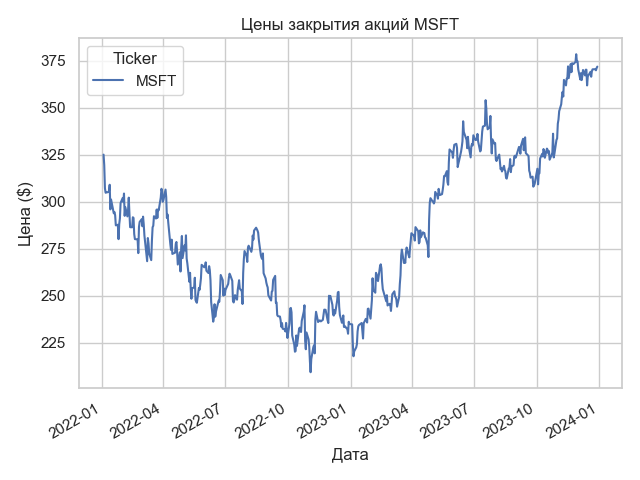
\includegraphics[width=0.65\textwidth]{MSFT_original_series.png}
    \caption{Исходный временной ряд}
\end{figure} \par

По данному ряду были построены разностные ряды первого и второго порядков:

\begin{figure}[h]
    \centering
    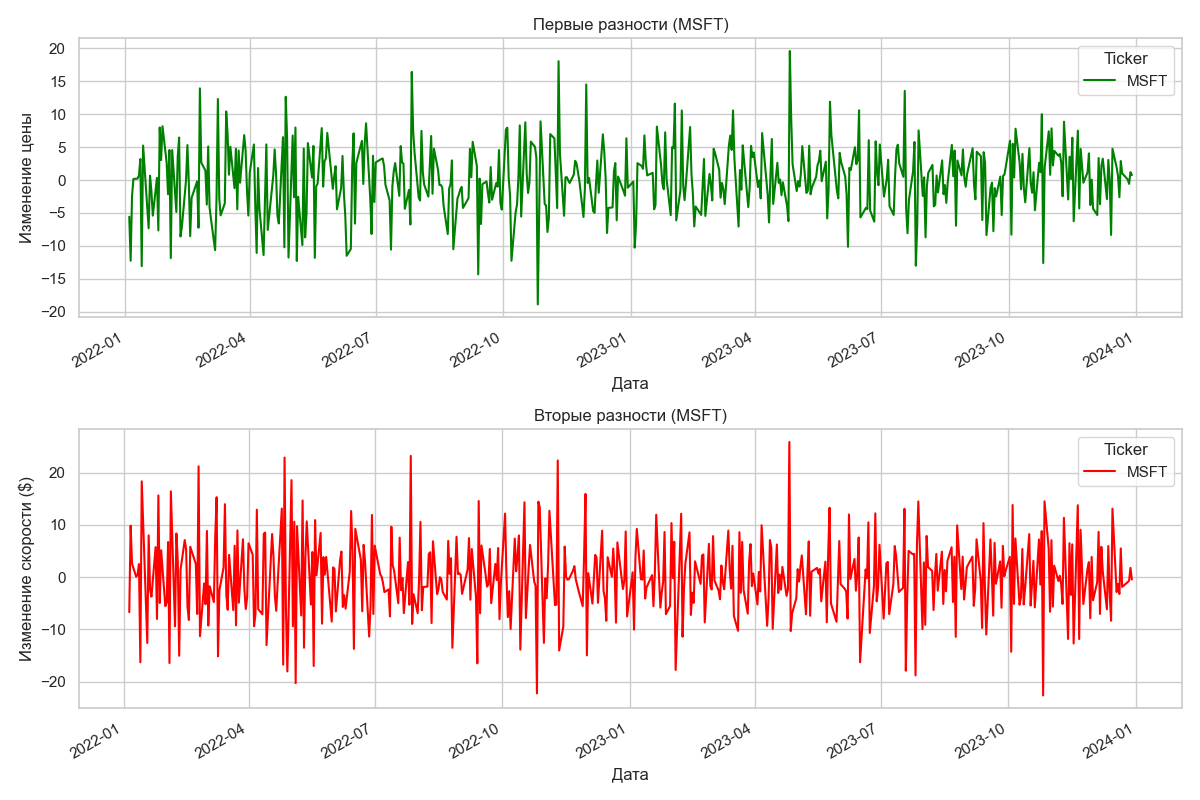
\includegraphics[width=0.6\textwidth]{MSFT_differencing.png}
    \caption{Разностные ряды}
\end{figure} \par

На основе данных рядов были построены разные АКФ:

\begin{figure}[h]
    \centering
    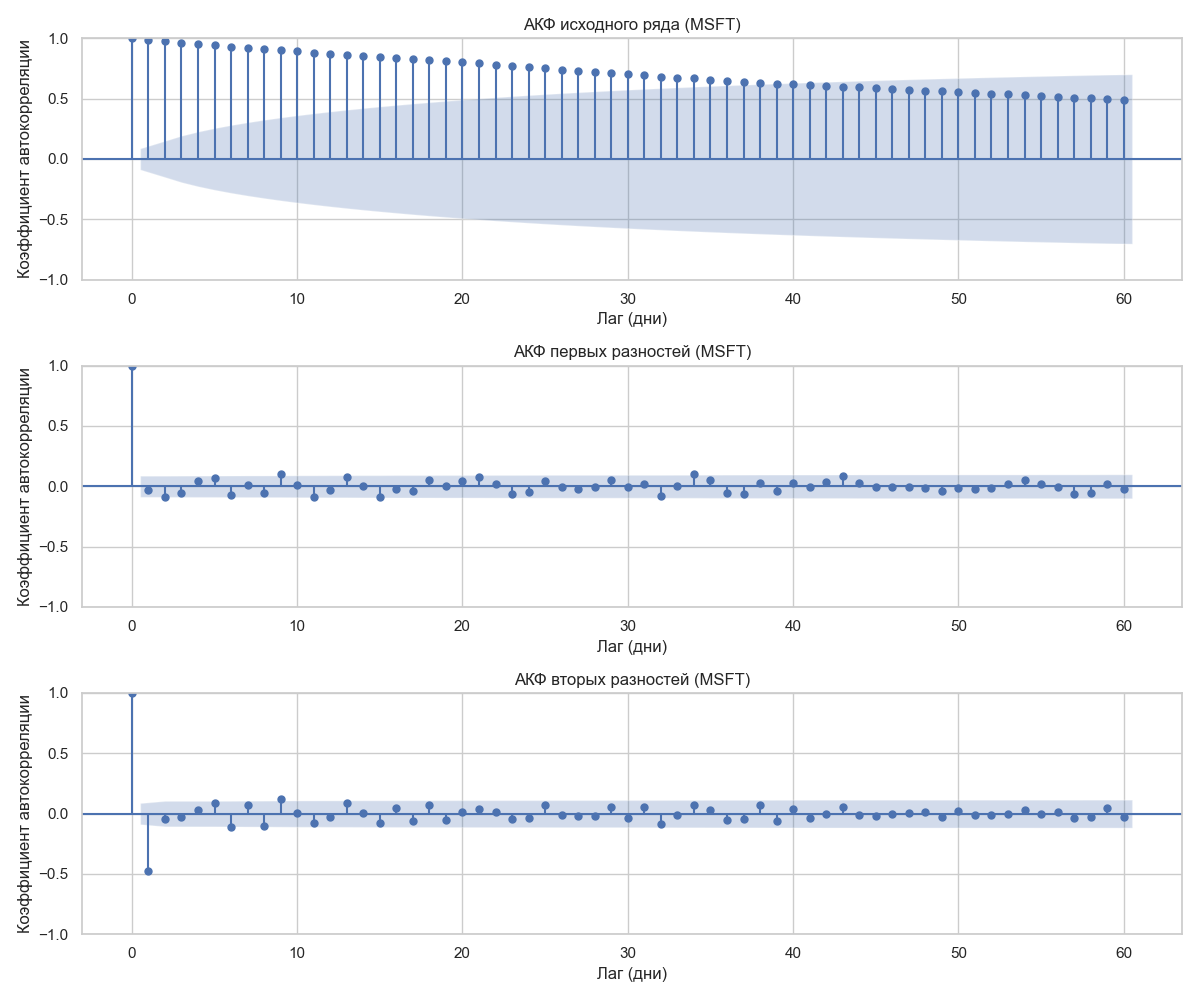
\includegraphics[width=0.45\textwidth]{MSFT_acf_analysis.png}
    \caption{АКФ для исходного ряда, разностного первого порядка и разностного второго порядка}
\end{figure} \par

На основе данного графика можно сделать несколько выводов:
\begin{itemize}
    \setlength{\itemsep}{0pt}
    \item Исходный ряд не стационарен, о чем свидетельствует отсутствие быстрого убывания в ноль столбцов функции;
    \item у исходного ряда присутсвует тренд;
    \item дифференцирование действительно убрало тренд из результирующих рядов, из-за чего ряды относительно стационарны;
    \item при построении разностного ряда второго порядка произошло "передифференцирование", из-за чего $\rho (1)$ 
    заметно отличается от разностного ряда первого порядка;
    \item сезонность выявить трудно: нет резких совпадающих пиков на графике исходного ряда.
\end{itemize}

На данных рядах был применен тест Дики-Фуллера для анализа стационарности:

\begin{figure}[h]
    \centering
    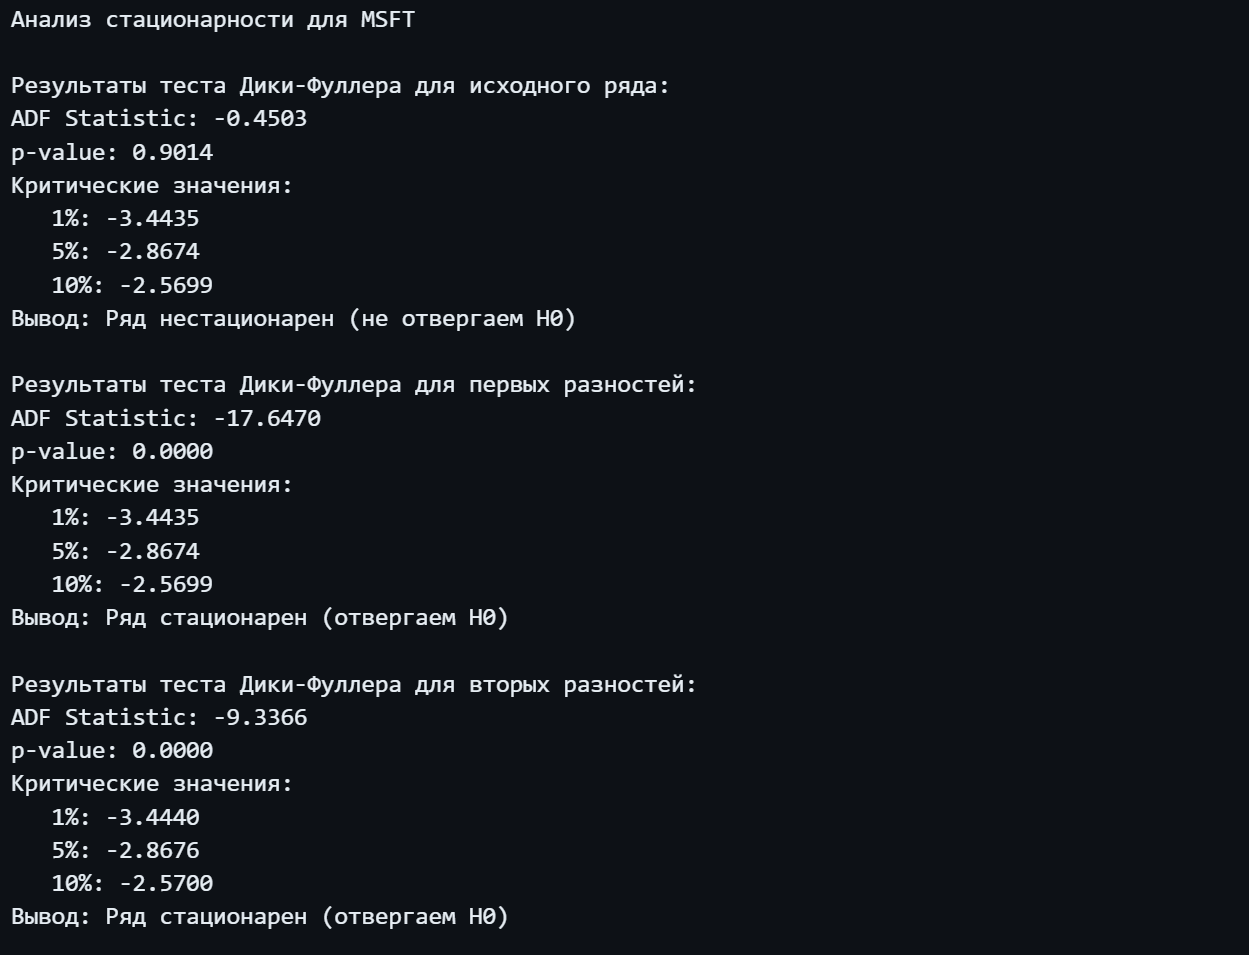
\includegraphics[width=0.45\textwidth]{MSFT_stationary_analysis_res.png}
    \caption{Результаты теста Дики-Фуллера для данных рядов}
\end{figure} \par

Как можно увидеть из результатов, ранние предположения оказались верными: исходный ряд нестационарен, 
что делает его менее пригодным для анализа, чем дифференцированные.\par
Наконец, были построены экспоненциальные сглаживания исходного ряда с разными коэффициентами памяти:

\begin{figure}[h]
    \centering
    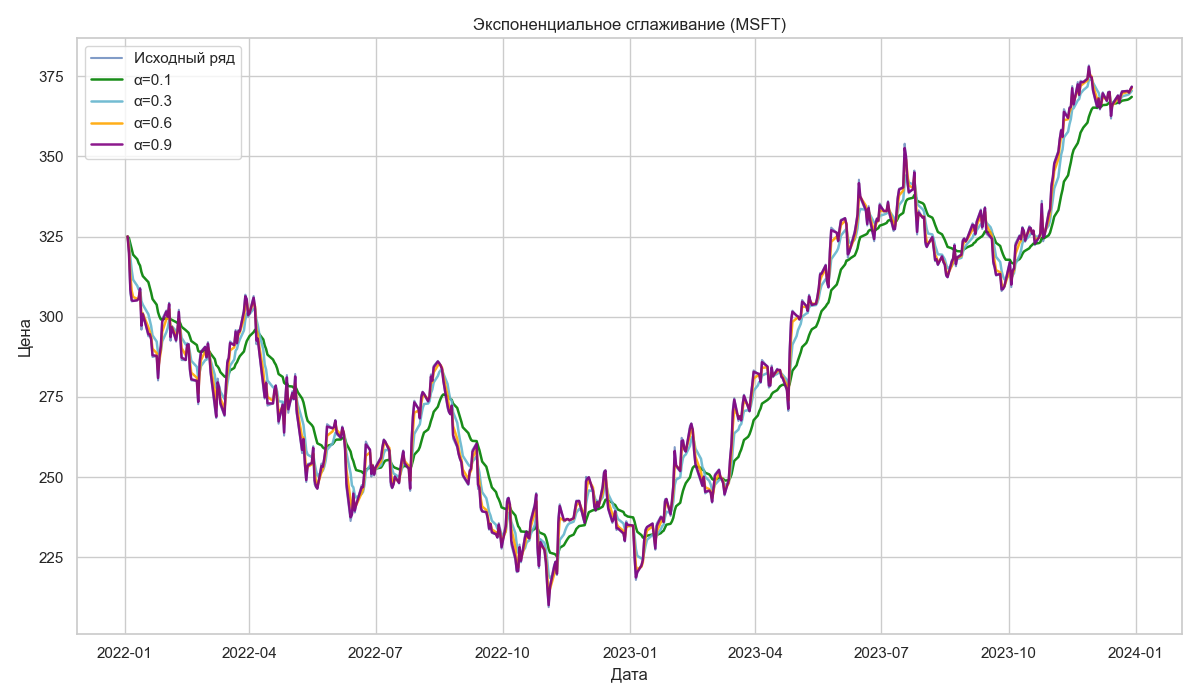
\includegraphics[width=0.65\textwidth]{MSFT_smoothing.png}
    \caption{Сглаживание исходного ряда}
\end{figure} \par

Как можно заметить, при малых значениях $\alpha$ шум убрался, при этом сохранились общие очертания 
исходного графика, что может быть полезно для визуализации и быстрого прогнозирования. При высоких значениях 
сильно заметны резкие колебания, что помогает замечать моментальные изменения, однако из-за этого прогнозирование 
и визуализация усложняются.

\chapter*{Заключение}
\addcontentsline{toc}{chapter}{Заключение}
\setcounter{chapter}{3}

В результате выполнения лабораторной работы мы познакомились с временными рядами и способами их анализа и преобразования. 
Применив теоретические знания на практике, мы провели анализ конкретного временного ряда акций компании и выявили 
определенные закономерности, а также смогли привести его к наиболее удобному для анализа виду.
\par
Знания и практический опыт, полученные во время выполнения работы, определенно понадобятся нам по профессии в будущем. 

\end{document}